% !TEX root = CSC104LectureNotes.tex

\setcounter{chapter}{0}
\chapter{Course Introduction}

\topquote{If I had an hour to solve a problem I'd spend 55 minutes thinking about the problem and 5 minutes thinking about solutions.}{Albert Einstein}

\minitoc

Welcome to {\color{mLightBrown}CSC 104: Programming Logic and Problem Solving!}  This course is intended for Information Technology majors, Computer Science majors, and anyone else who's interested in learning about computer programming and about computer programmers.

\section{Course Strategies}

Two personality traits that seem to be common to successful programmers are:
\begin{itemize}
\item Curiosity
\item Perseverance
\end{itemize}

Why is that?  Many computer programmers spend a lot of time solving problems that have never been solved before.  This often requires thinking about an old problem in a new way, and deciding not to give up.

Also, sometimes the best result is not a complete answer, but just an answer that's incrementally better than the most recent answer.  Small successes are successes, and we must accept them and celebrate them!  Sometimes programmers talk about being \textbf{productively lost} -- not quite sure which way to proceed, but at least having a good understanding of the problem one is in.

For these reasons, it is important that you \textbf{ask lots of questions}, during class, in your professor's office hours, or over electronic communication.  Every question moves the conversation, and aids in problem solving.  Even asking a ``bad'' question helps eliminate an avenue of inquiry that might not have led to success.

Related to this idea, it's important that you \textbf{answer every question} during class or on homework.  Even if your answer is wrong or incomplete, a ``bad'' answer is something you can build upon.

Make sure to \textbf{review what you've learned} after every class, and make sure everything makes sense.  Ask questions as soon as you have to, in order to get back on track.

Finally, make sure you understand your professor's policies.  \textbf{Read the syllabus} and understand your responsibilities, and what's expected of you.  Check on when things like exams are expected to happen, and add them to your calendar now.

\section{Daily Preview}

Each day, your professor will display a slide like this:
\begin{myfigure}{Typical Lecture Introduction Slide}
	%\caption
	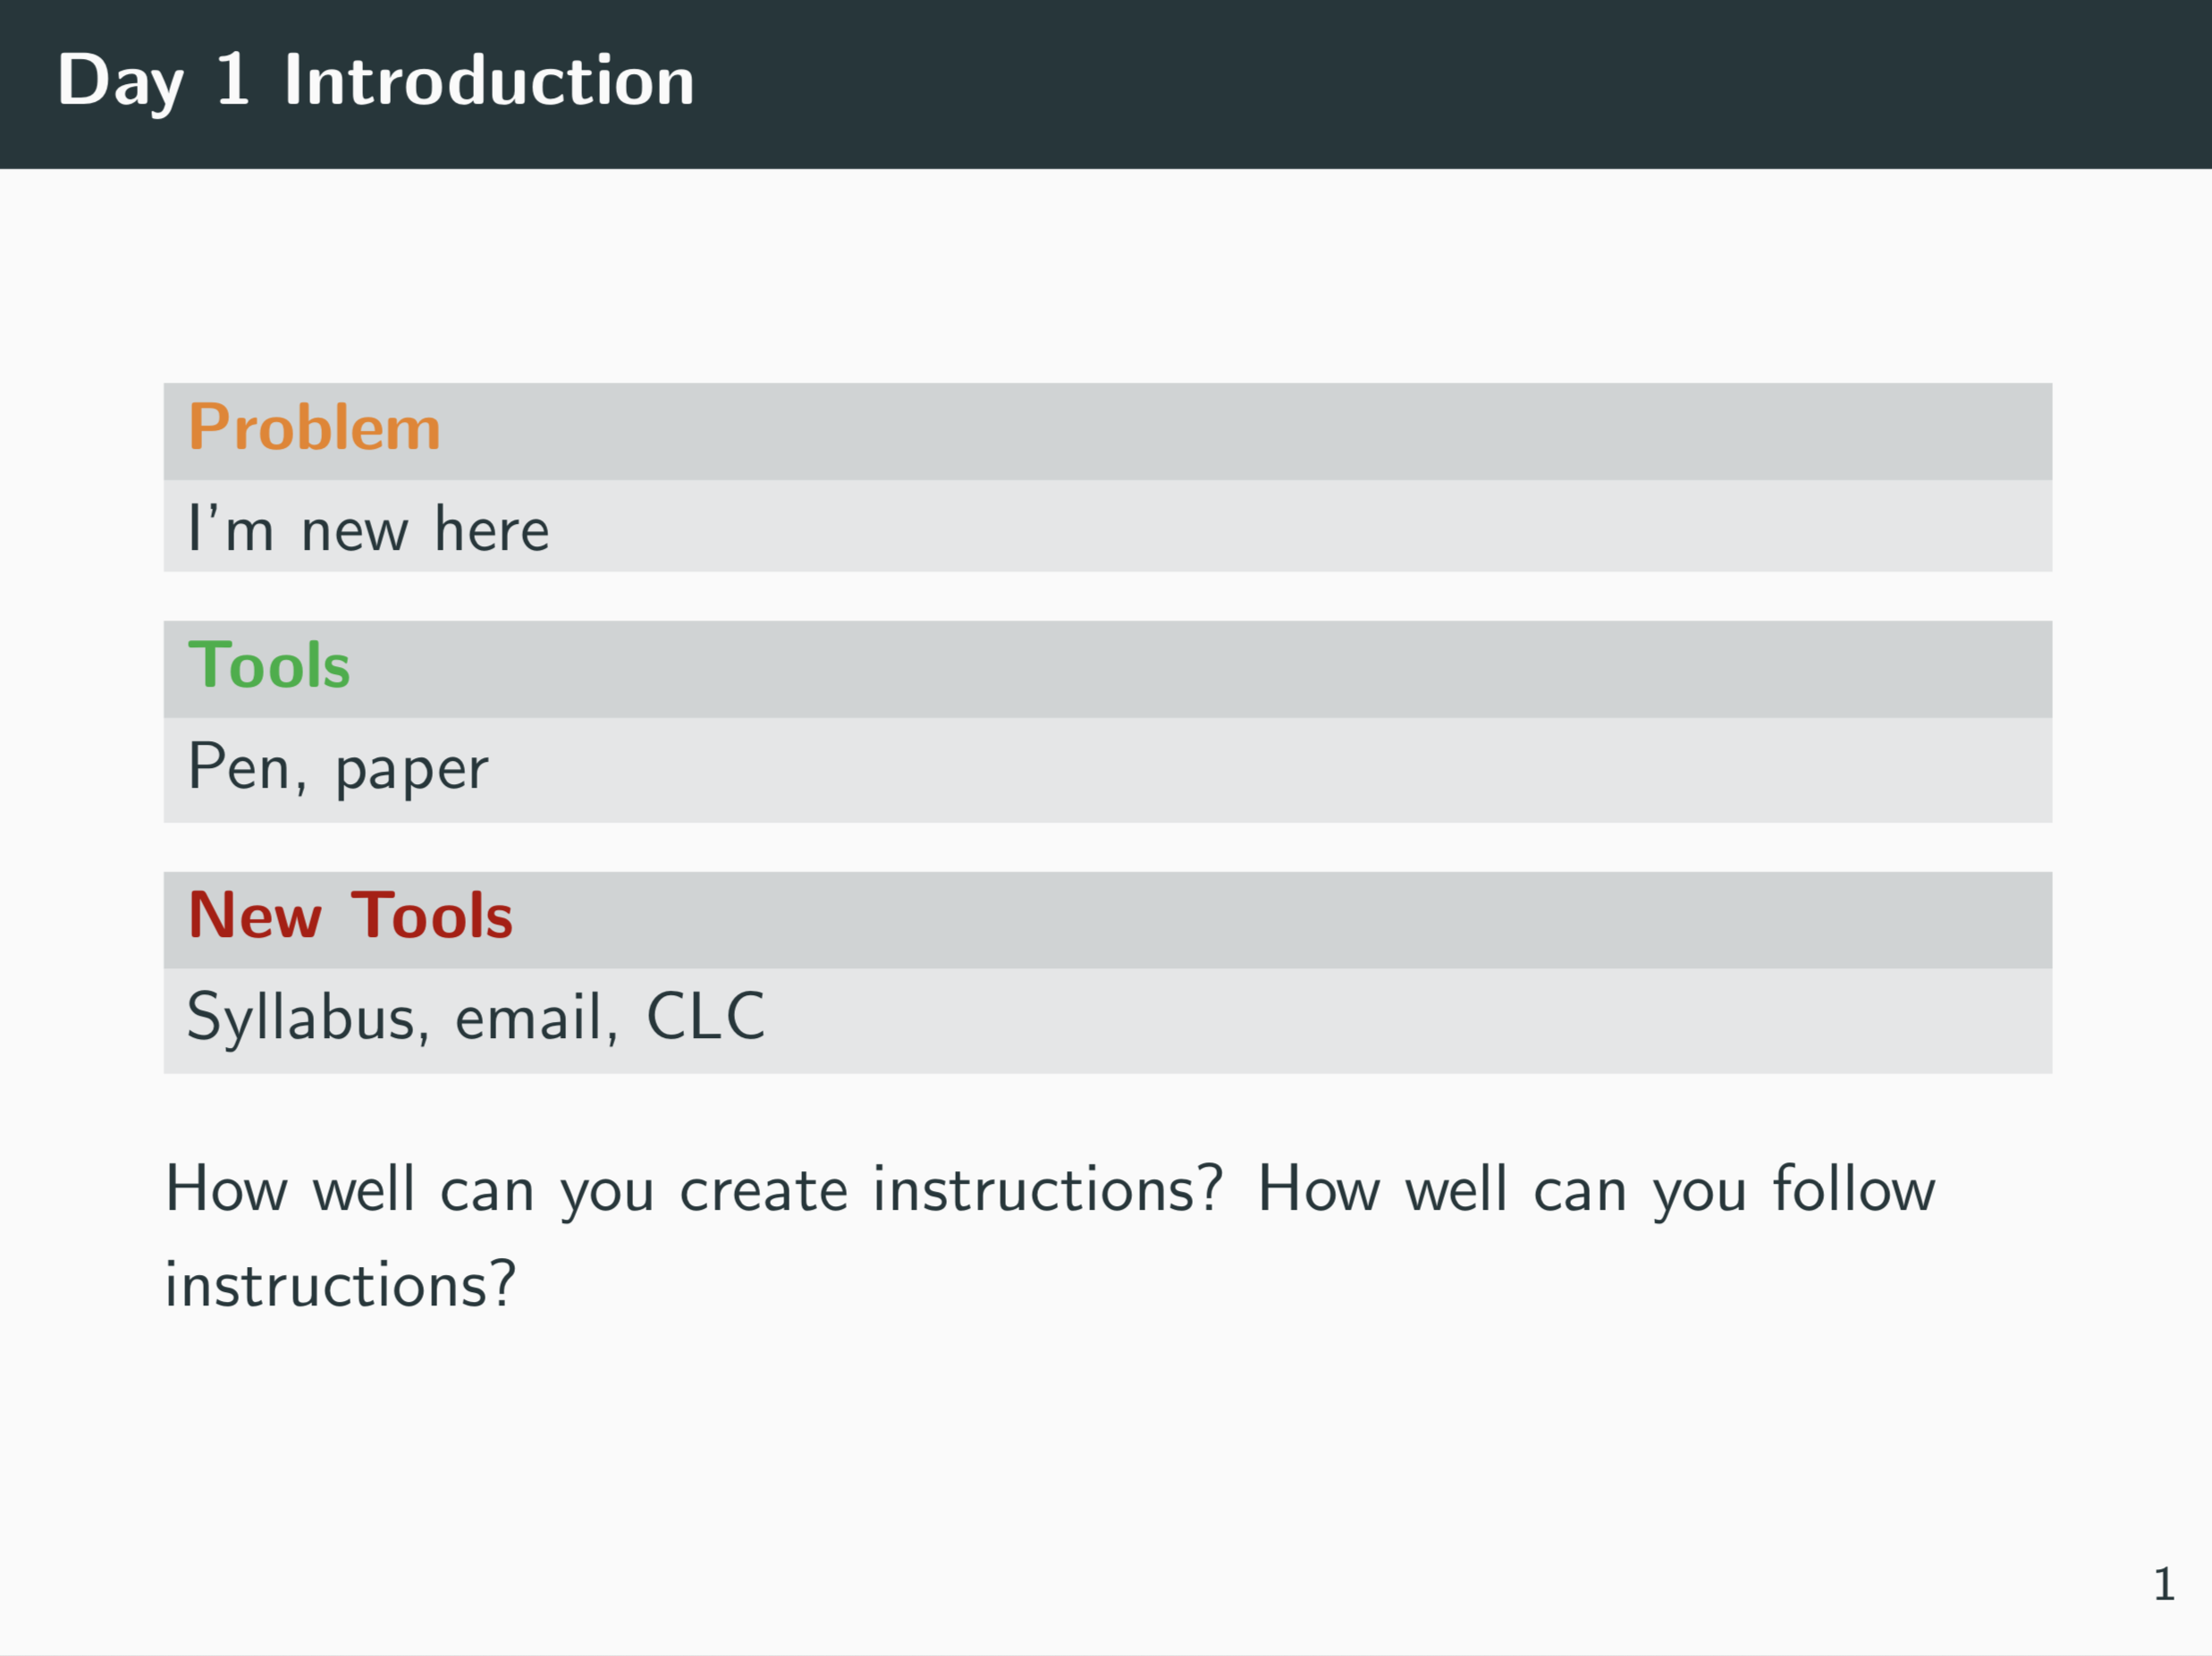
\includegraphics[scale=0.25]{day1slide}
\end{myfigure}

Understanding the day's problem, tools to be used, and new tools to be acquainted with, is a good way to get into the right mindset for the day's activities.

\section{Interview Questions}

It was once very popular for hiring officers to ask programmers to solve very difficult logic puzzles during job interviews.  These questions are no longer used so frequently, but they were popular because, it was thought, they allowed the interviewers to see how the interview subjects think about new problems.  As we work through the first part of this course, we will examine questions like this, to try to gain insight into how programmers think, and why it seems that programmers think about things in a different way than other people do.

The article that begins on Page \pageref{cnn} at the end of today's notes describes the situation well.

\section{Logo Exercise}

The best way to learn how to do anything is to do it.  Several times this semester, you will be engaging in a hands-on activity, meant to help you enhance a skill that you will be relying on throughout the rest of the course.  Today, you will learn just how difficult it can be to write directions and to follow them.

\section{Homework}

For homework, make sure you do the following things:
\begin{itemize}
\item Sign up for any web sites your professor asked you to sign up for, like the course management system, communications tools, etc.
\item Purchase access to the zyBooks textbook
\item Familiarize yourself with the location of the Computer Learning Center in B 225
\end{itemize}

\newpage
\label{cnn}
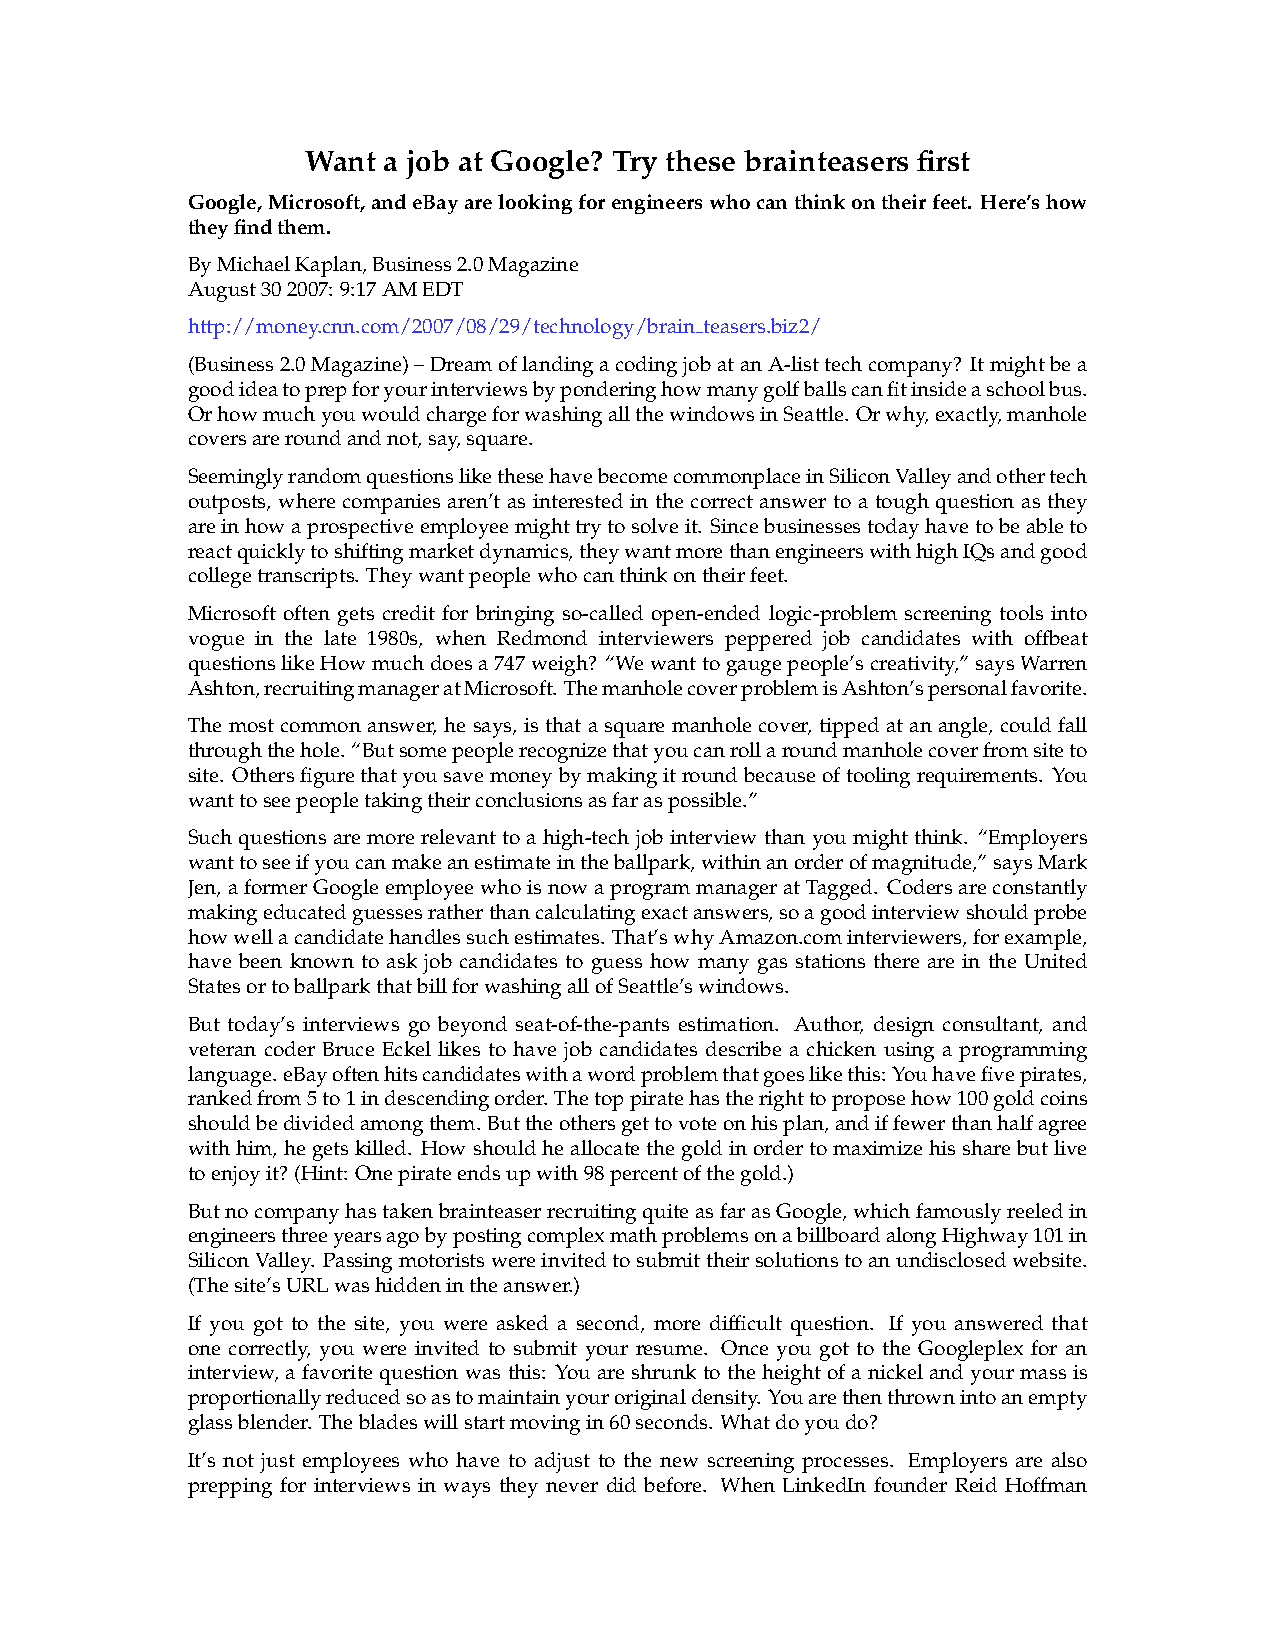
\includepdf[pages=-,pagecommand={\pagestyle{fancy}},noautoscale,scale=0.9]{day1-interview-article.pdf}
